\documentclass[]{article}
\usepackage{lmodern}
\usepackage{amssymb,amsmath}
\usepackage{ifxetex,ifluatex}
\usepackage{fixltx2e} % provides \textsubscript
\ifnum 0\ifxetex 1\fi\ifluatex 1\fi=0 % if pdftex
  \usepackage[T1]{fontenc}
  \usepackage[utf8]{inputenc}
\else % if luatex or xelatex
  \ifxetex
    \usepackage{mathspec}
    \usepackage{xltxtra,xunicode}
  \else
    \usepackage{fontspec}
  \fi
  \defaultfontfeatures{Mapping=tex-text,Scale=MatchLowercase}
  \newcommand{\euro}{€}
\fi
% use upquote if available, for straight quotes in verbatim environments
\IfFileExists{upquote.sty}{\usepackage{upquote}}{}
% use microtype if available
\IfFileExists{microtype.sty}{%
\usepackage{microtype}
\UseMicrotypeSet[protrusion]{basicmath} % disable protrusion for tt fonts
}{}
\usepackage[margin=1in]{geometry}
\usepackage{graphicx}
\makeatletter
\def\maxwidth{\ifdim\Gin@nat@width>\linewidth\linewidth\else\Gin@nat@width\fi}
\def\maxheight{\ifdim\Gin@nat@height>\textheight\textheight\else\Gin@nat@height\fi}
\makeatother
% Scale images if necessary, so that they will not overflow the page
% margins by default, and it is still possible to overwrite the defaults
% using explicit options in \includegraphics[width, height, ...]{}
\setkeys{Gin}{width=\maxwidth,height=\maxheight,keepaspectratio}
\ifxetex
  \usepackage[setpagesize=false, % page size defined by xetex
              unicode=false, % unicode breaks when used with xetex
              xetex]{hyperref}
\else
  \usepackage[unicode=true]{hyperref}
\fi
\hypersetup{breaklinks=true,
            bookmarks=true,
            pdfauthor={Reza},
            pdftitle={Applying for the data science position},
            colorlinks=true,
            citecolor=blue,
            urlcolor=blue,
            linkcolor=magenta,
            pdfborder={0 0 0}}
\urlstyle{same}  % don't use monospace font for urls
\setlength{\parindent}{0pt}
\setlength{\parskip}{6pt plus 2pt minus 1pt}
\setlength{\emergencystretch}{3em}  % prevent overfull lines
\setcounter{secnumdepth}{0}

%%% Use protect on footnotes to avoid problems with footnotes in titles
\let\rmarkdownfootnote\footnote%
\def\footnote{\protect\rmarkdownfootnote}

%%% Change title format to be more compact
\usepackage{titling}

% Create subtitle command for use in maketitle
\newcommand{\subtitle}[1]{
  \posttitle{
    \begin{center}\large#1\end{center}
    }
}

\setlength{\droptitle}{-2em}
  \title{Applying for the data science position}
  \pretitle{\vspace{\droptitle}\centering\huge}
  \posttitle{\par}
  \author{Reza}
  \preauthor{\centering\large\emph}
  \postauthor{\par}
  \predate{\centering\large\emph}
  \postdate{\par}
  \date{March 16, 2016}



\begin{document}

\maketitle


Dear

I am writing to express my interest in working with zapier as data
scientist. I am doing the last steps of my doctorate in mathematics. I
have been doing research and teaching in the my field of study from the
time I was doing my master. Alongside I did cooperate with experts in
other fields including economists and urban planners.

To name some, I developed an algorithm for assessing accessibility in
cities using big graphs and programmed it in MatLab. I am familiar with
by nature statistical techniques of remote sensing as well, and help
urban planners running them. With economists, we studied financial
derivatives with aim of understanding their nature and their
relationship with gambling. Also I designed a data bank for their
scientific papers.

I would like to enter the business sector and found the data analysis
really interesting and perfectly fitted to my theoretical background. I
am a good independent fast leaner. During the last couple of months I
learned SQL and R programming and using it in data analysis. Plus I
already am familiar with Python and would like to learn it more deeply.

You can find some works of mine in my \href{github.com/srhumir}{github
account}

In R I love the ``dplyr''" and ``data.table'' packages for their fast
and efficient capability of cleaning and summarizing the data.
``raster'' is a very nice package for working with grid ?data?. For
plotting one should not underestimate the base plotting system of R but
whenever it is too much coding needed using it, I prefer to use
``ggplot2''. Rmarkdown in combination with LaTex is a great tool for
making reports. In machine learning techniques, neural network is really
good however sometimes I found it is too slow. Random forest worked
quite good.

\subsubsection{Explanation of a work}\label{explanation-of-a-work}

MODIS is a satellite which provide mainly two kind of products. First
land surface temperature (LST) and second Normalized Difference
Vegetation Index (NDVI), an index between -1 and 1 of which higher
values indicate indicate more dense vegetation. This data are provided
in weekly intervals. Its problem is that it is really coerce, with
resolution of 960m for LST. On the other hand we had an image of the
SPOT satellite of 1.5m resolution which unfortunately does not provide
LST information but fortunately provides enough data for computing NDVI.
It is known that NDVI and LST have an inverse relationship. We use this
fact to compute LST for SPOT.

Briefly I computed two linear models. One to convert NDVI of SPOT to
NDVI of MODIS and another to convert NDVI to LST. The first one is quite
straightforward. But the second model had to be based on not all pixels
but just the so called hot edge pixels. i.e.~pixels which are among the
hottest 5 percent when NDVI is binned in 0.3 unit intervals. Scatter
plot below shows NDVI vs LST. Red dots are hot edges and green dots
indicates the fitted linear model.

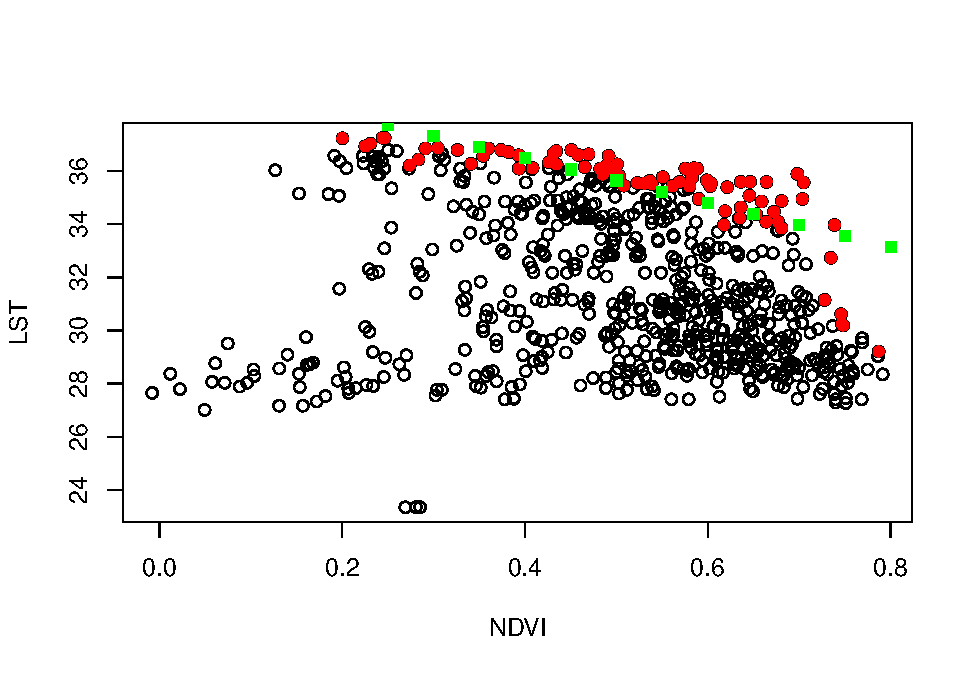
\includegraphics{zapier_files/figure-latex/unnamed-chunk-1-1.pdf}

To refine the results, I used the fact that the temperature of a point
is dependent to its surrounding points. To take into account this fact,
I computed the residuals of the model above with respect to all pixels.
Then trained a neural network with with NDVI of each pixel and its eight
suroonding pixels as input and the pixels residual as output.

As I agree that my resume might not be yet convincing for you to give me
a full job, I would like to propose a two-month unpaid remote trainee
program. I would do the jobs you expect from a data analyst. I am sure I
can rapidly learn whatever needed for the job and I haven't learned yet.
After two month I would have a job or at least a priceless experience
working with your company.

Enclosed please find my resume. I am looking forward to hearing from you
and ready to start from April.

With highest regards

Reza Hosseini

\end{document}
